%%%%%%%%%%%%%%%%%%%%%%%%%%%%%%%%%%%%%%%%%%%%%%%%%%%%%%%%%%%%%%%%%%%%%
%% This is a (brief) model paper using the achemso class
%% The document class accepts keyval options, which should include
%% the target journal and optionally the manuscript type.
%%%%%%%%%%%%%%%%%%%%%%%%%%%%%%%%%%%%%%%%%%%%%%%%%%%%%%%%%%%%%%%%%%%%%
\documentclass[journal=esthag,manuscript=article, layout=traditional, email=true]{achemso} %,layout=twocolumn
\SectionNumbersOn
%%%%%%%%%%%%%%%%%%%%%%%%%%%%%%%%%%%%%%%%%%%%%%%%%%%%%%%%%%%%%%%%%%%%%
%% Place any additional packages needed here.  Only include packages
%% which are essential, to avoid problems later.
%%%%%%%%%%%%%%%%%%%%%%%%%%%%%%%%%%%%%%%%%%%%%%%%%%%%%%%%%%%%%%%%%%%%%
\usepackage{chemformula} % Formula subscripts using \ch{}
\usepackage[T1]{fontenc} % Use modern font encodings
\usepackage[utf8]{inputenc}
\usepackage{enumitem} % Allow enumeration to resume
\usepackage[normalem]{ulem} % Strike-through text
%
% *** ACRONYM PACKAGES ***
\usepackage[acronym]{glossaries}
\newacronym{eDNA}{eDNA}{environmental DNA}
\newacronym{UAV}{UAV}{unmanned aerial vehicle}
\newacronym{RC}{RC}{remote controller}
\newacronym{BVLOS}{BVLOS}{beyond visual line of sight}
\newacronym{GLM}{GLM}{generalized linear model}
\newacronym{MOTU}{MOTU}{molecular operational taxonomic unit}
%
% *** Links ***
\usepackage{hyperref}
%
% *** Units ***
\usepackage{siunitx}
%
% *** Tables ***
\usepackage{booktabs}
\usepackage[table]{}
\usepackage{makecell}
%%%%%%%%%%%%%%%%%%%%%%%%%%%%%%%%%%%%%%%%%%%%%%%%%%%%%%%%%%%%%%%%%%%%%
%% If issues arise when submitting your manuscript, you may want to
%% un-comment the next line.  This provides information on the
%% version of every file you have used.
%%%%%%%%%%%%%%%%%%%%%%%%%%%%%%%%%%%%%%%%%%%%%%%%%%%%%%%%%%%%%%%%%%%%%
%%\listfiles
%
%%%%%%%%%%%%%%%%%%%%%%%%%%%%%%%%%%%%%%%%%%%%%%%%%%%%%%%%%%%%%%%%%%%%%
%% Place any additional macros here.  Please use \newcommand* where
%% possible, and avoid layout-changing macros (which are not used
%% when typesetting).
%%%%%%%%%%%%%%%%%%%%%%%%%%%%%%%%%%%%%%%%%%%%%%%%%%%%%%%%%%%%%%%%%%%%%
\newcommand*\mycommand[1]{\texttt{\emph{#1}}}
%
%%%%%%%%%%%%%%%%%%%%%%%%%%%%%%%%%%%%%%%%%%%%%%%%%%%%%%%%%%%%%%%%%%%%%
%% Meta-data block
%% ---------------
%% Each author should be given as a separate \author command.
%%
%% Corresponding authors should have an e-mail given after the author
%% name as an \email command. Phone and fax numbers can be given
%% using \phone and \fax, respectively; this information is optional.
%%
%% The affiliation of authors is given after the authors; each
%% \affiliation command applies to all preceding authors not already
%% assigned an affiliation.
%%
%% The affiliation takes an option argument for the short name.  This
%% will typically be something like "University of Somewhere".
%%
%% The \altaffiliation macro should be used for new address, etc.
%% On the other hand, \alsoaffiliation is used on a per author basis
%% when authors are associated with multiple institutions.
%%%%%%%%%%%%%%%%%%%%%%%%%%%%%%%%%%%%%%%%%%%%%%%%%%%%%%%%%%%%%%%%%%%%%
% Change font sizes to make it fit on page
\renewcommand*\affilsize{\footnotesize}
\renewcommand*\authorsize{\large}
\renewcommand*\emailsize{\normalsize}
\renewcommand*\titlesize{\LARGE}
%
\author{Steffen Kirchgeorg}
\affiliation[ERL]{Environmental Robotics Laboratory, ETH Zürich, Zürich, 8092, Switzerland}
\alsoaffiliation[WSL]{Swiss Federale Institute for Forest, Snow and Landscape Research WSL, Birmensdorf, 8903, Switzerland}
\email{skirchgeorg@ethz.ch}
%
\author{Jia Jin Marc Chang}
\affiliation[NUS]{Department of Biological Sciences, National University of Singapore, Singapore, 117558, Singapore}
\alsoaffiliation[LKC]{Lee Kong Chian Natural History Museum, National University of Singapore, Singapore, 117377, Singapore}
%
\author{Yin Cheong Aden Ip}
\affiliation[WA]{School of Marine and Environmental Affairs, University of Washington, Seattle, Washington, 98105, United States of America}
%
\author{Meret Jucker}
\affiliation[EDNA]{Environmental DNA, ETH Zürich, Zürich, 8092, Switzerland}
%
\author{Christian Geckeler}
\affiliation[ERL]{Environmental Robotics Laboratory, ETH Zürich, Zürich, 8092, Switzerland}
\alsoaffiliation[WSL]{Swiss Federale Institute for Forest, Snow and Landscape Research WSL, Birmensdorf, 8903, Switzerland}
%
\author{Martina Lüthi}
\affiliation[ELE]{Ecosystems and Landscape Evolution, ETH Zürch, Zürich, 8092, Switzerland}
%
\author{Enrico van der Loo}
\affiliation[EDNA]{Environmental DNA, ETH Zürich, Zürich, 8092, Switzerland}
%
\author{Elvira Mächler}
\affiliation[SimpleX]{SimplexDNA AG, Winterthur, 8404, Switzerland}
%
\author{Nicolás D. Franco-Sierra}
\affiliation[SYN]{Syndesis Health, Palm Beach Gardens, Florida, 33408, United States of America}
%
\author{Mailyn Adriana Gonzalez Herrera}
\affiliation[HUM]{Alexander von Humboldt Biological Resources Research Institute, Bogotá, 111311, Colombia}
%
\author{Lo\"{i}c Pellissier}
\affiliation[ELE]{Ecosystems and Landscape Evolution, ETH Zürch, Zürich, 8092, Switzerland}
\alsoaffiliation[WSL]{Swiss Federale Institute for Forest, Snow and Landscape Research WSL, Birmensdorf, 8903, Switzerland}
%
\author{Kristy Deiner}
\affiliation[EDNA]{Environmental DNA, ETH Zürich, Zürich, 8092, Switzerland}
\alsoaffiliation[SimpleX]{SimplexDNA AG, Winterthur, 8404, Switzerland}
%
\author{Andrea Desiderato}
\affiliation[PL]{Department of Invertebrate Zoology and Hydrobiology, Faculty of Biology and Environmental Protection, University of Lodz, Lodz, 90-136, Poland}
%
\author{Stefano Mintchev}
\affiliation[ERL]{Environmental Robotics Laboratory, ETH Zürich, Zürich, 8092, Switzerland}
\alsoaffiliation[WSL]{Swiss Federale Institute for Forest, Snow and Landscape Research WSL, Birmensdorf, 8903, Switzerland}
%
%%%%%%%%%%%%%%%%%%%%%%%%%%%%%%%%%%%%%%%%%%%%%%%%%%%%%%%%%%%%%%%%%%%%%
%% The document title should be given as usual. Some journals require
%% a running title from the author: this should be supplied as an
%% optional argument to \title.
%%%%%%%%%%%%%%%%%%%%%%%%%%%%%%%%%%%%%%%%%%%%%%%%%%%%%%%%%%%%%%%%%%%%%
\title[eProbe]{eProbe: Sampling of Environmental DNA within Tree Canopies with Drones}
%
%%%%%%%%%%%%%%%%%%%%%%%%%%%%%%%%%%%%%%%%%%%%%%%%%%%%%%%%%%%%%%%%%%%%%
%% Some journals require a list of abbreviations or keywords to be
%% supplied. These should be set up here, and will be printed after
%% the title and author information, if needed.
%%%%%%%%%%%%%%%%%%%%%%%%%%%%%%%%%%%%%%%%%%%%%%%%%%%%%%%%%%%%%%%%%%%%%
\abbreviations{
eDNA, environmental DNA;
RC, remote controller;
BVLOS, beyond visual line of sight;
UAV, unmanned aerical vehicle;
COI, cytochrome c oxidase subunit I;
GLM, generalized linear model;
}

\keywords{biodiversity, eDNA, surface swabbing, done-based sampling}
%

% Add * in front of email for corresponding author
\makeatletter
\patchcmd{\acs@contact@details}{E}{*\,E}{}{}
\patchcmd{\acs@email@list@aux}{;}{\par*\,Email}{}{} % added <<<<<<<<<<<<
\makeatother
%%%%%%%%%%%%%%%%%%%%%%%%%%%%%%%%%%%%%%%%%%%%%%%%%%%%%%%%%%%%%%%%%%%%%
%% The manuscript does not need to include \maketitle, which is
%% executed automatically.
%%%%%%%%%%%%%%%%%%%%%%%%%%%%%%%%%%%%%%%%%%%%%%%%%%%%%%%%%%%%%%%%%%%%%
\begin{document}
%
\centering 
\section*{Supplementary Information}
Summary: 6 Pages (S1-S6), 1 Table (S1) and 6 Figures (S1-S6) 

\renewcommand{\thepage}{S\arabic{page}}

% Reset counter
\setcounter{figure}{0}
\renewcommand{\thefigure}{S\arabic{figure}}

\setcounter{table}{0}
\renewcommand{\thetable}{S\arabic{table}}

\begin{table}[tbh]
  \footnotesize
  \centering
  \caption{Results of the PERMANCOVA. Conc: DNA concentration; Time: Day or Night.}
    \begin{tabular}{lccccc}
        \toprule
        Terms & Df & SumOfSqs & R2 & F & Pr(>F) \\
        \midrule
        Conc & 1 & 0.6019 & 0.15968 & 1.5402 & 0.005 \\
        Time & 1 & 0.4320 & 0.1146 & 1.1053 & 0.205 \\
        Residual & 7 & 2.7357 & 0.72572 & - \\
        Total & 9 & 3.7696 & 1 & - \\
        \bottomrule
    \end{tabular}%
    \label{tab:s1-permancova}
\end{table}

\begin{figure}[tbh]
    \centering
    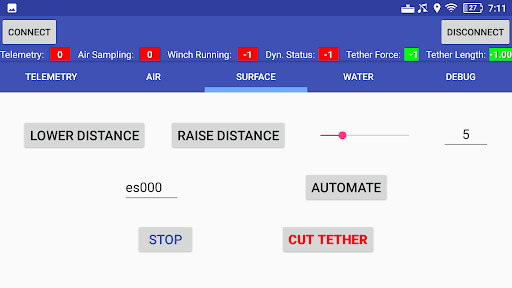
\includegraphics[width=0.7\linewidth]{figures/S1_GUI.png}
    \caption{Custom GUI for DJI remote controller to select probing depth (in meters), the call to "automate" to lower and raise the probe automatically as well as the option to stop and cut the tether. Winch box feedback is shown at the top bar (winch status, dynamixel status, tether force and tether length).}
    \label{fig:s0-gui}
\end{figure}

\begin{figure}[tbh]
    \centering
    \includegraphics[width=\linewidth]{figures/s2_xprize_map.png}
    \caption{Surface sample locations within the XPRIZE Rainforest Semi-Finals Competition Area (red) in Singapore with the base station outside the competition area.}
    \label{fig:s1-sample-location}
\end{figure}



\begin{figure}[tbh]
    \centering
    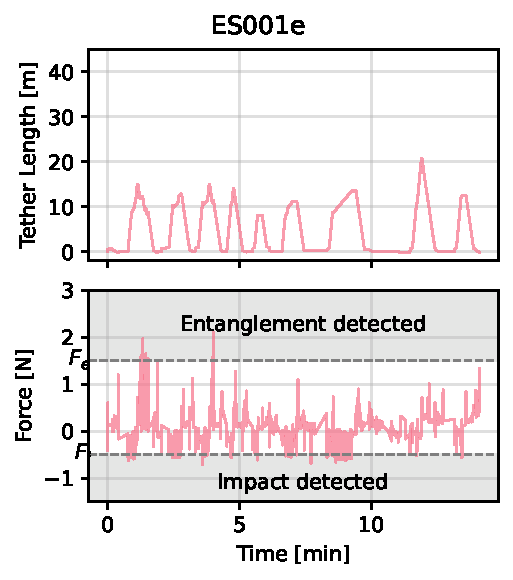
\includegraphics[width=0.32\linewidth]{figures/probe_ES001e.pdf}
    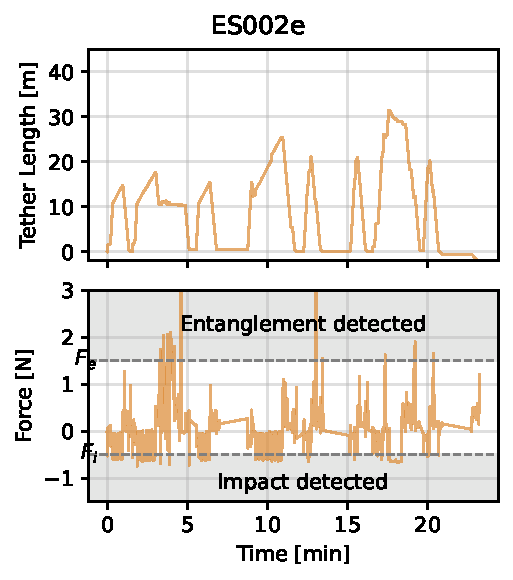
\includegraphics[width=0.32\linewidth]{figures/probe_ES002e.pdf}
    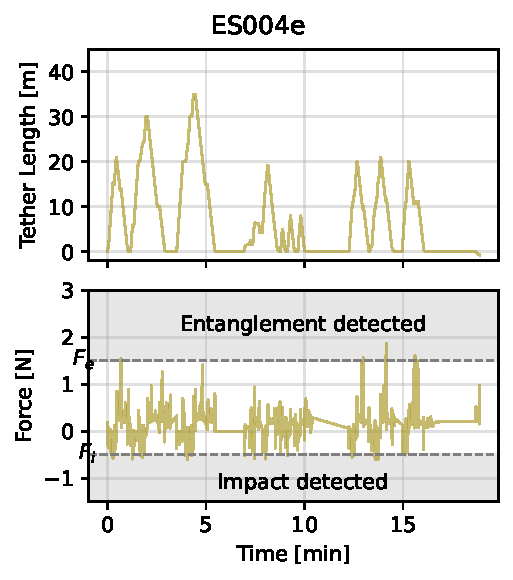
\includegraphics[width=0.32\linewidth]{figures/probe_ES004e.pdf}
    \\
    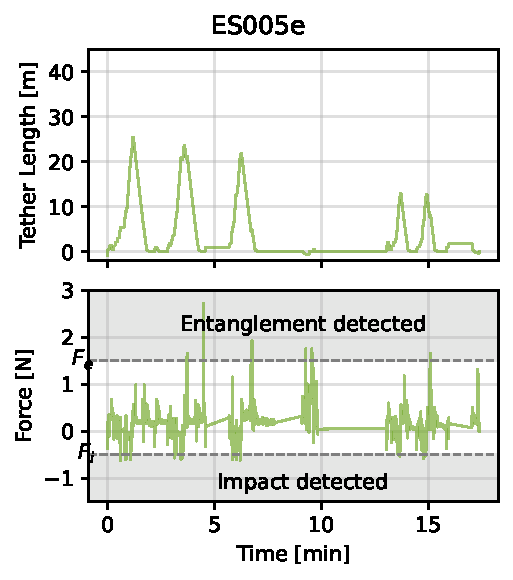
\includegraphics[width=0.32\linewidth]{figures/probe_ES005e.pdf}
    \includegraphics[width=0.32\linewidth]{figures/probe_ES006e.pdf}
    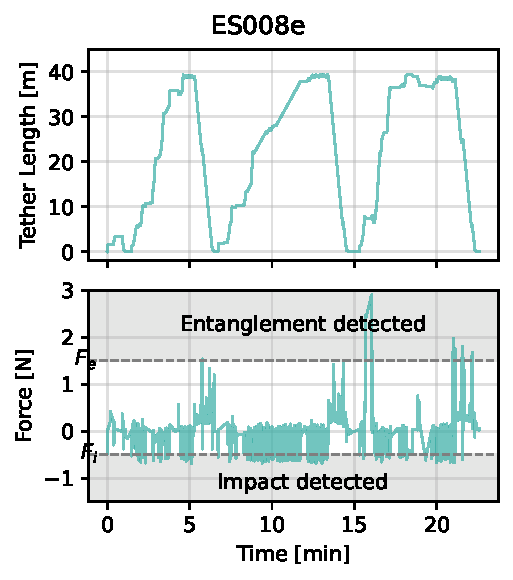
\includegraphics[width=0.32\linewidth]{figures/probe_ES008e.pdf}
    \\
    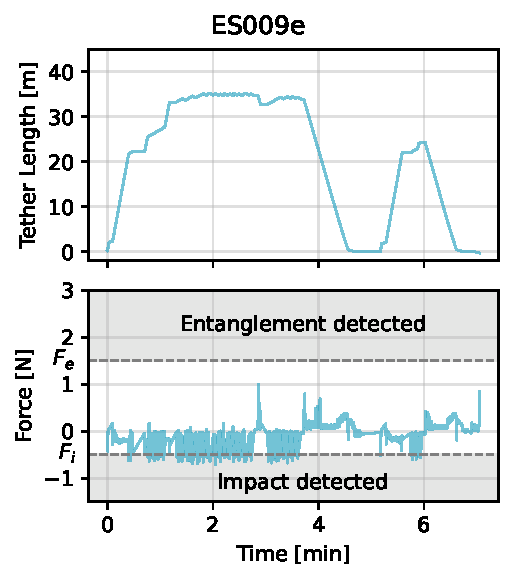
\includegraphics[width=0.32\linewidth]{figures/probe_ES009e.pdf}
    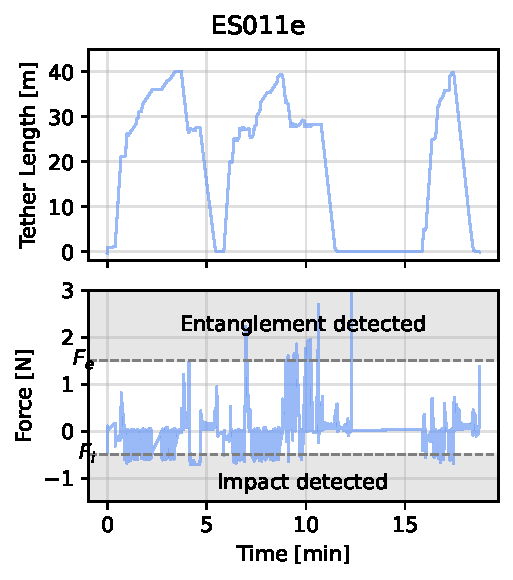
\includegraphics[width=0.32\linewidth]{figures/probe_ES011e.pdf}
    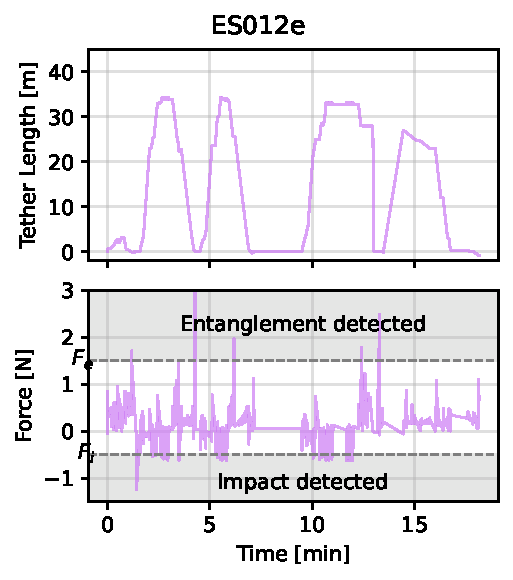
\includegraphics[width=0.32\linewidth]{figures/probe_ES012e.pdf}
    \caption{Tether Length and Force for: ES001e, ES002e, ES004e, ES005e, ES006e, ES008e, ES009e, ES011e, ES012e. Probes ES007e and ES0010e were not deployed. Data logging issues occurred during deployment of ES003e.}
    \label{fig:s2-metadata}
\end{figure}

\begin{figure}[tbh]
    \centering
    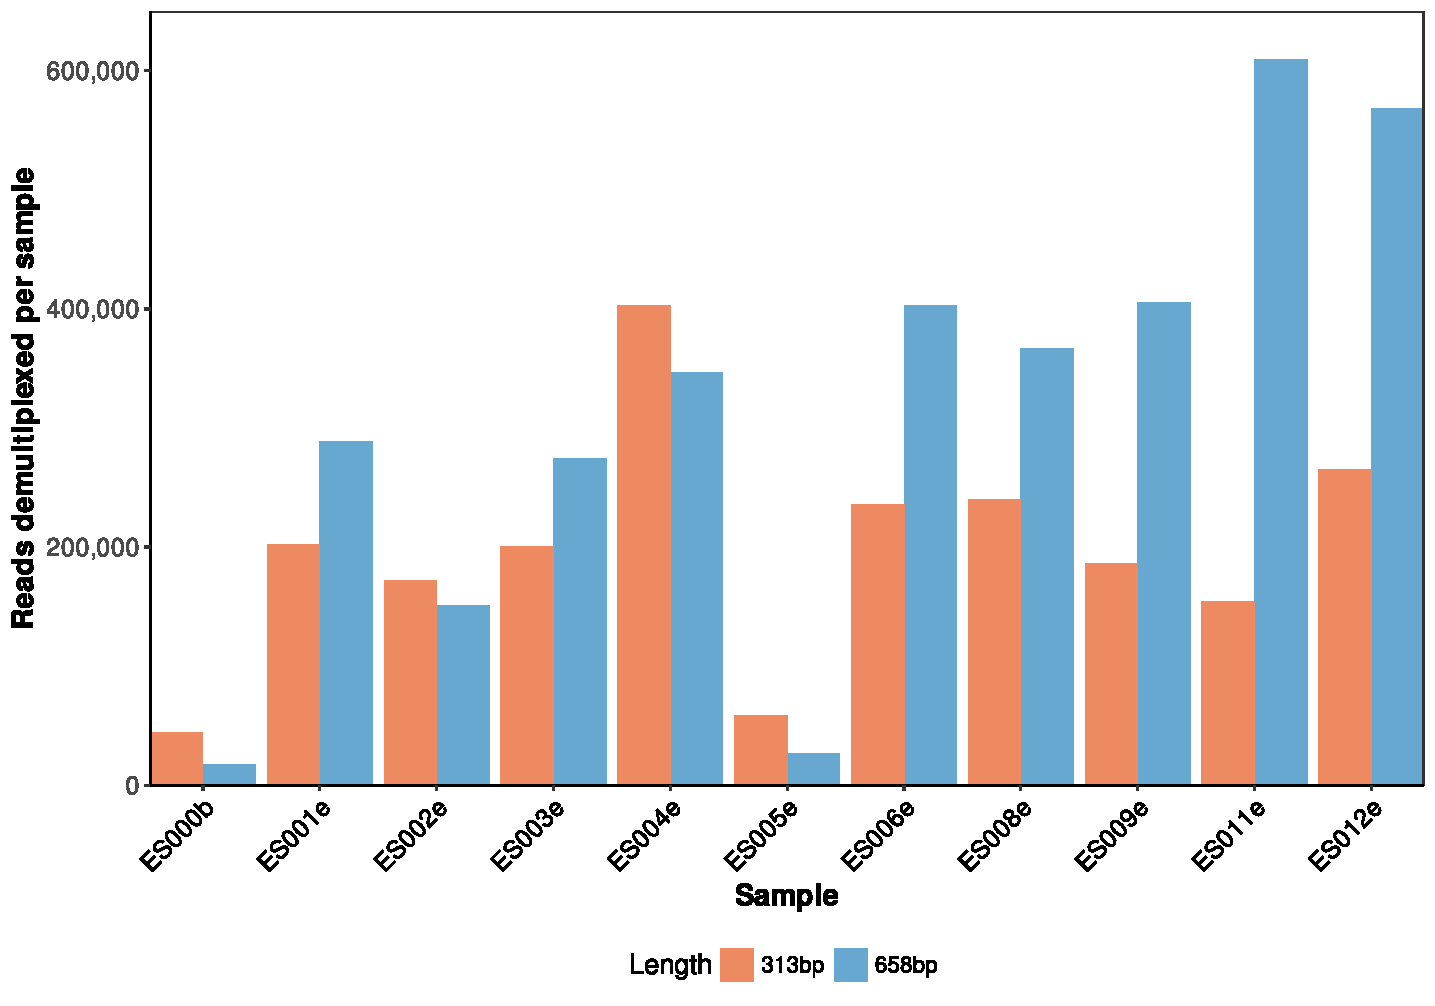
\includegraphics[width=0.75\linewidth]{figures/S4_demult_barplot.pdf}
    \caption{Number of demultiplexed reads per sample, per COI length amplicon.}
    \label{fig:s3-reads}
\end{figure}

\begin{figure}[tbh]
    \centering
    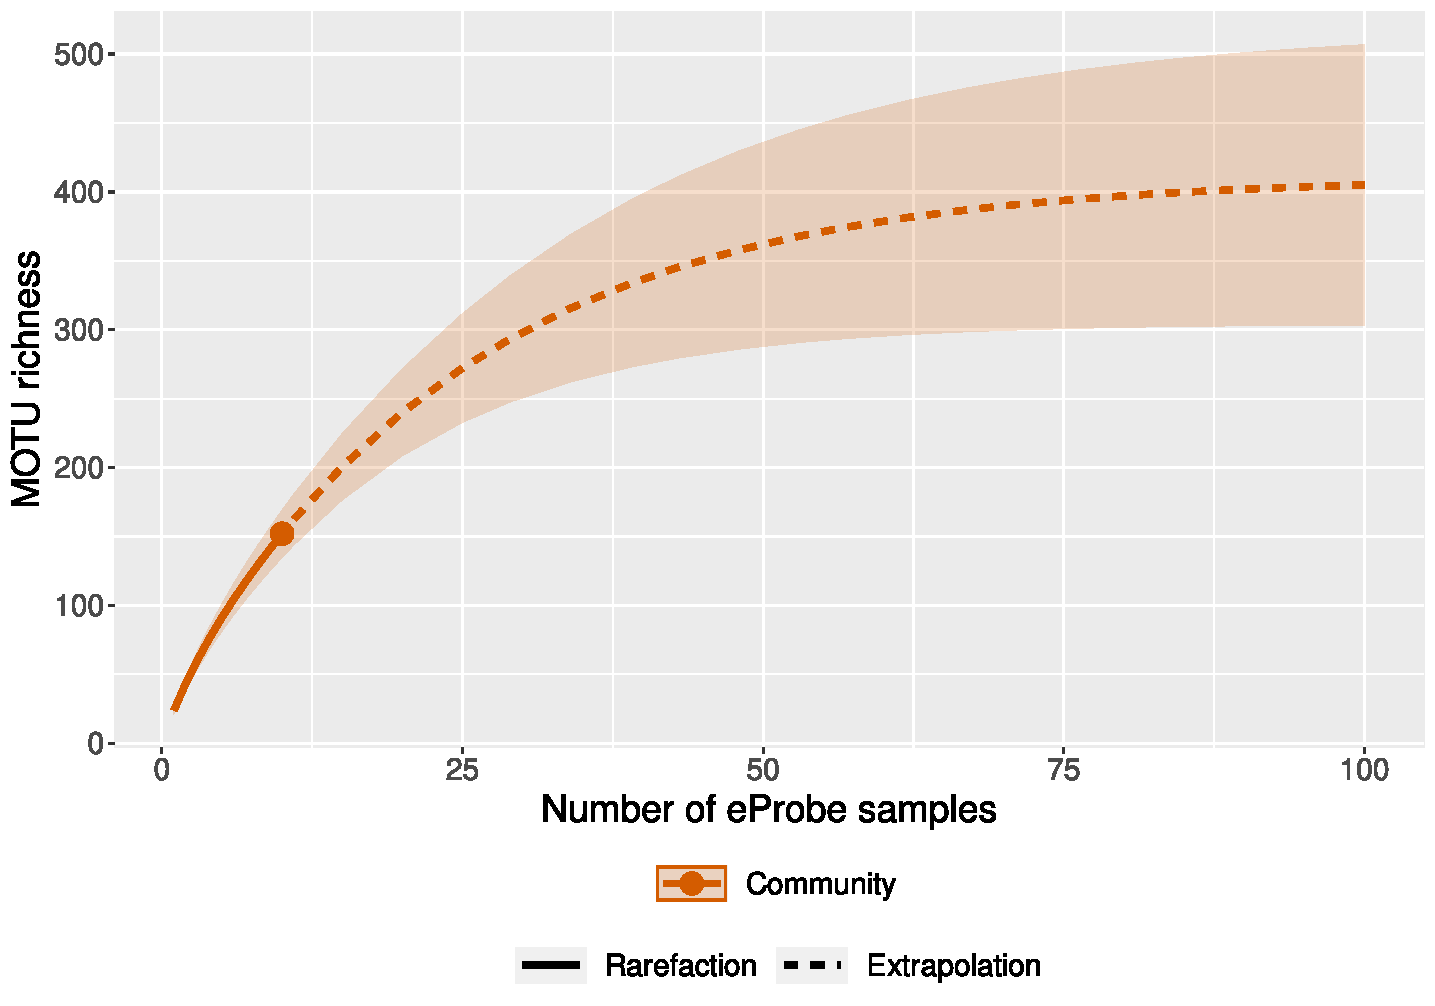
\includegraphics[width=0.75\linewidth]{figures/S5_species_accum_curve.pdf}
    \caption{Species accumulation curve showing the relationship between number of eProbe samples and MOTU richness of Central Catchment Nature Reserve, Singapore, analyzed with iNEXT. Dotted lines show projected values and shaded areas indicate 95 \% confidence intervals.}
    \label{fig:s4-accumulation}
\end{figure}

\begin{figure}[tbh]
    \centering
    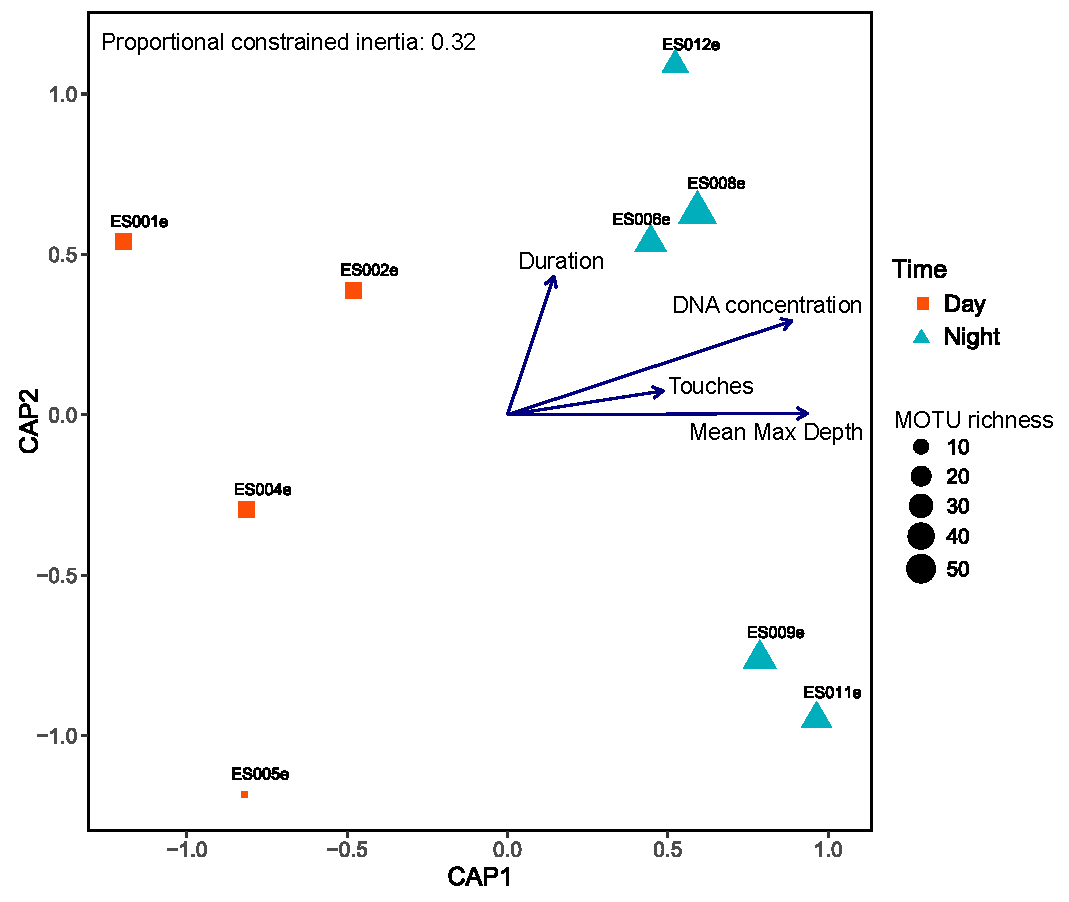
\includegraphics[width=0.75\linewidth]{figures/S6_dbRDA_mod.pdf}
    \caption{Biplot of the distance-based redundancy analysis of the species detected (Jaccard similarity) associated with the sampling parameters, including duration, touches and mean/max depth as well as the time of sampling. The length of the arrows is proportional to the effect of the constraining variable. MOTU composition recovered was different between day and night.}
    \label{fig:s5-dbra}
\end{figure}

\end{document}